% \documentclass[twocolumn]{aastex6}
\documentclass{aastex6}

\newcommand{\radmc}{\texttt{RADMC-3D}}
\newcommand{\kms}{ \textrm{km s}^{-1} }
\newcommand{\todo}[1]{ \textcolor{red}{#1}}
\newcommand{\vt}{ {\bm \theta}}
\newcommand{\msun}{M$_\odot$}

\newcommand{\twelve}{CO}
\newcommand{\thirteen}{${}^{13}$CO}
\newcommand{\eighteen}{C${}^{18}$O}

\begin{document}

\title{GW Ori: A Massive Stellar Systems with a Circum-triple Disk, Caught Young Ages}
\author{I.~Czekala\altaffilmark{1}, S.~M.~Andrews\altaffilmark{1}, et al.} % E.~L.~N.~Jensen\altaffilmark{2}, K.~G.~Stassun\altaffilmark{3,4}, G.~Torres\altaffilmark{1}, \& D.~J.~Wilner\altaffilmark{1}}
\altaffiltext{1}{Harvard-Smithsonian Center for Astrophysics,
			 60 Garden Street, Cambridge, MA 02138; \email{iczekala@cfa.harvard.edu}}
\altaffiltext{2}{Department of Physics and Astronomy, Swarthmore College, 500 College Avenue, Swarthmore, PA 19081}
\altaffiltext{3}{Department of Physics and Astronomy, Vanderbilt University, Nashville, TN 37235}
\altaffiltext{4}{Department of Physics, Fisk University, Nashville, TN 37208}

\begin{abstract}
We present spatially and spectrally resolved Atacama Large Millimeter/submillimeter Array (ALMA) observations of gas and dust in the disk orbiting the pre-main sequence triple GW Ori.
\end{abstract}
\keywords{ protoplanetary disks -- stars: fundamental parameters -- stars: pre-main sequence -- stars: individual (GW Ori)}


\section{Introduction -- {\bf Keivan} \label{sec:intro}}

\noindent
{\bf Keivan's things to explore:}
\begin{itemize}
\item Nominal periods: AB = 240d, C = 4000d.
\item Evolution of 5 Msun star from PMS tracks?? What age constraints are there from 5 Msun with late-G spectral type?
\item Where does the nominal 5 Myr age for lambda Ori come from (see Dolan papers)?
\item Is position and gamma velocity consistent with lambda Ori membership? Could it be in foreground Ori association?
\item Other systems that are HAeBe primary, T Tauri secondary, and tertiary -- or main sequence equivalents? (Nominal masses are 5, 0.5, 0.5 Msun). See Maxwell Moe papers (B stars with TTS companions).
\item Dimmings like RW Aur, with associated RV deviations --- Shevchenko papers.
\item KELT dimmings??
\item There is a parallax and also proper motions.
\item Tertiary has been seen by Berger et al 2011... flux ratios.
\item Fang 2014 -- VLT spectra, accretion line diagnostics, SED modeling, disk wind? Gap flows.
\item X-ray source?
\end{itemize}

Orbit calculation \citep{mathieu91}.

H-band interferometry, resolved orbit \citep{berger11}.

Spectroscopic activity and inner disk clearing \citep{fang14}.

\section{Observations and Data Reduction}

\subsection{Millimeter Interferometry}

ALMA Cycle II program to observe spectroscopic binaries. Observed on XX. Very bright disk, detected in \twelve, \thirteen, and \eighteen. Peak line fluxes are XX. Line widths are XX.

\begin{figure*}[htb]
\begin{center}
  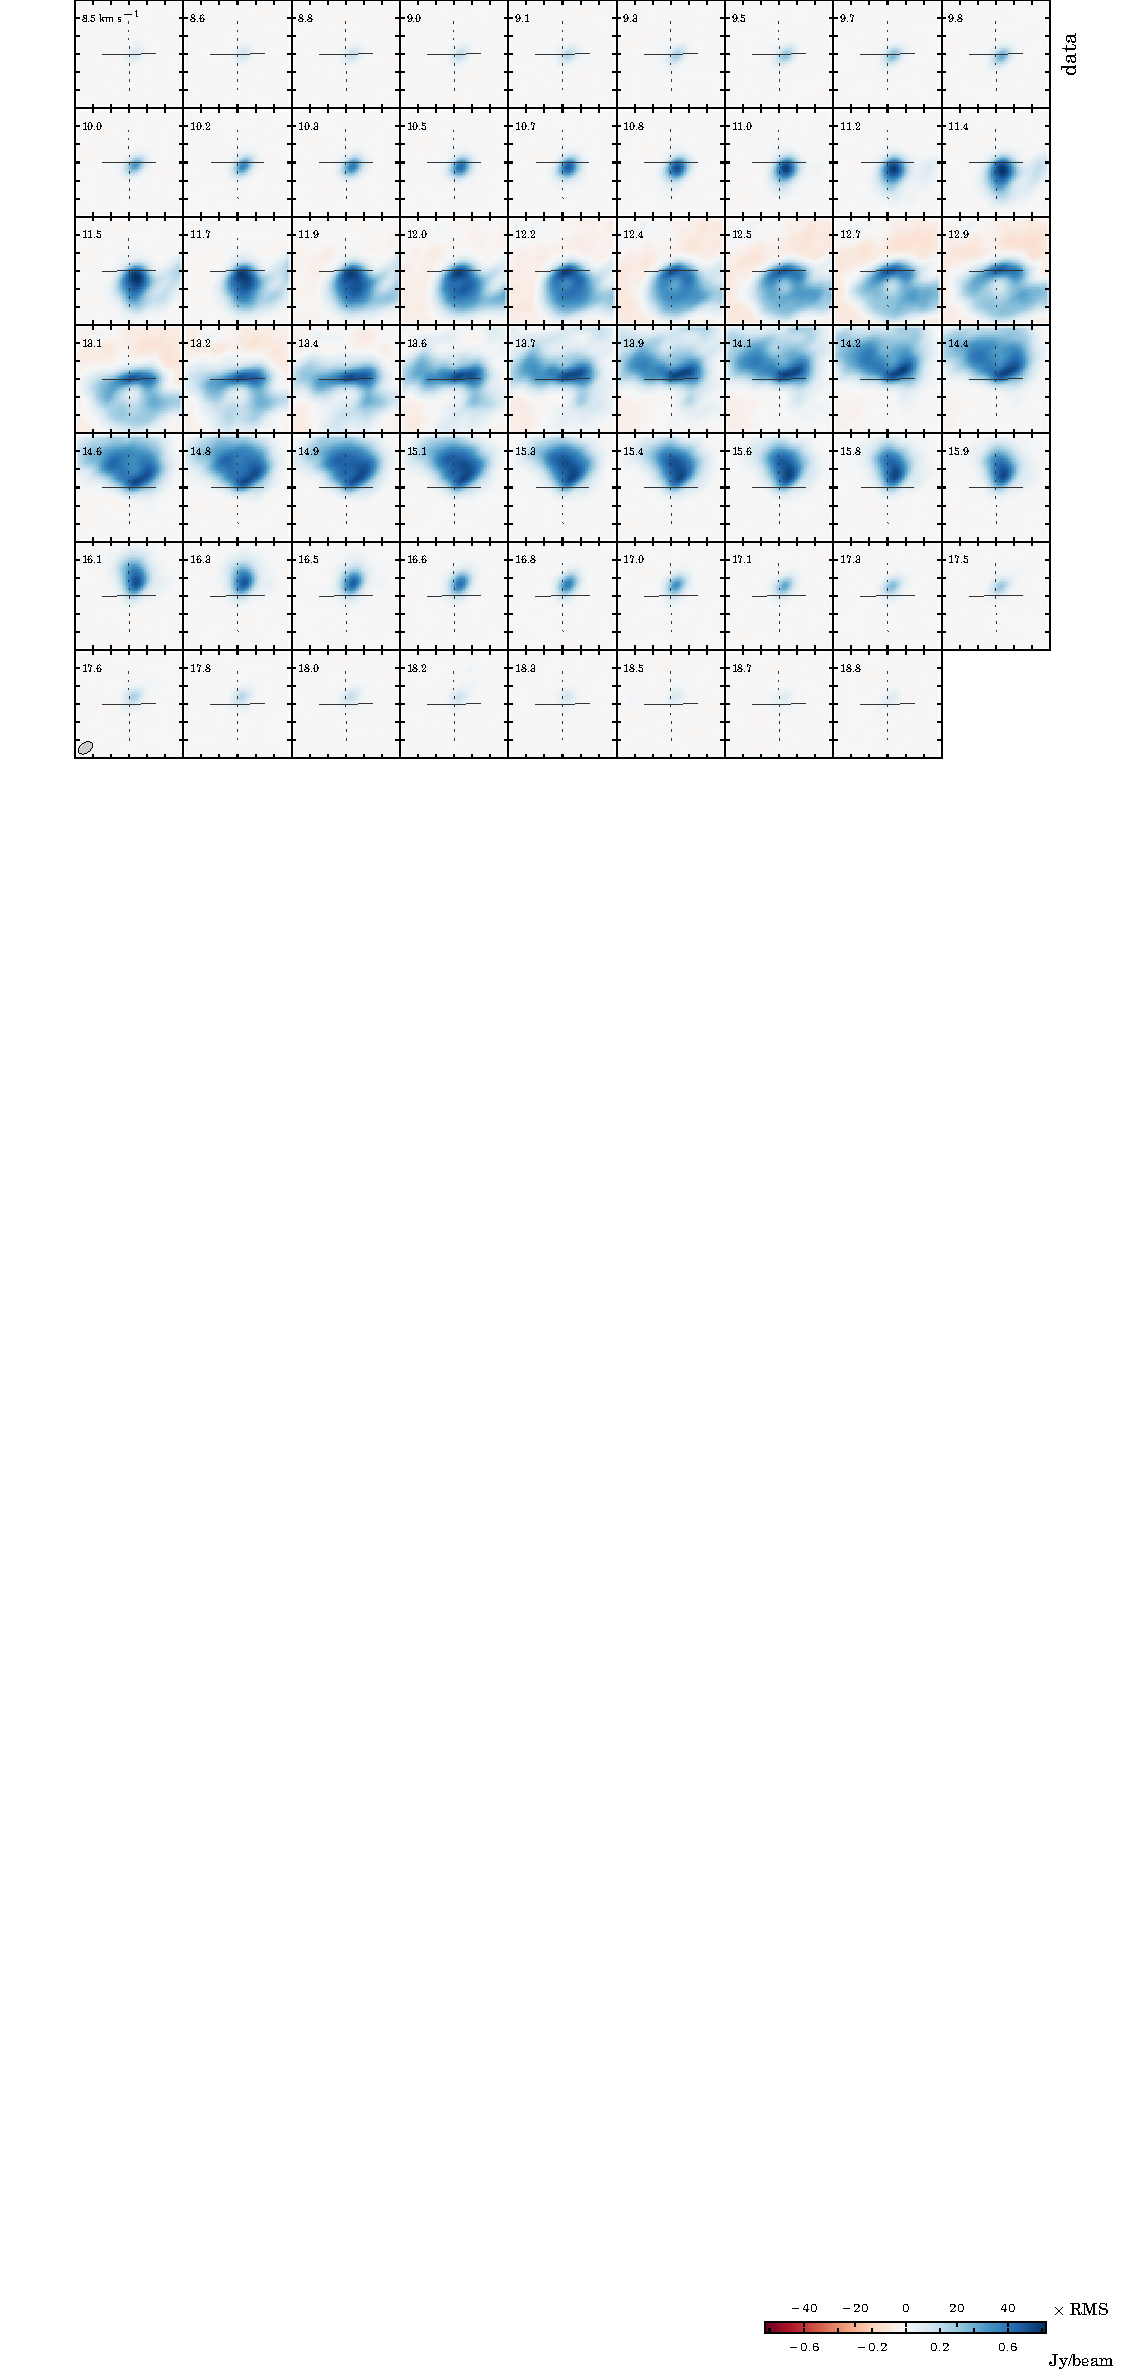
\includegraphics[draft,width=\textwidth,height=0.9\textheight]{chmaps_CO.pdf}
  \figcaption{\twelve\ channel maps. Due to the nearby cloud contamination, we do not model these. (Or, we model only the XX channels.)
  \label{fig:chmaps_CO}}
  \end{center}
\end{figure*}

\begin{figure*}[htb]
\begin{center}
  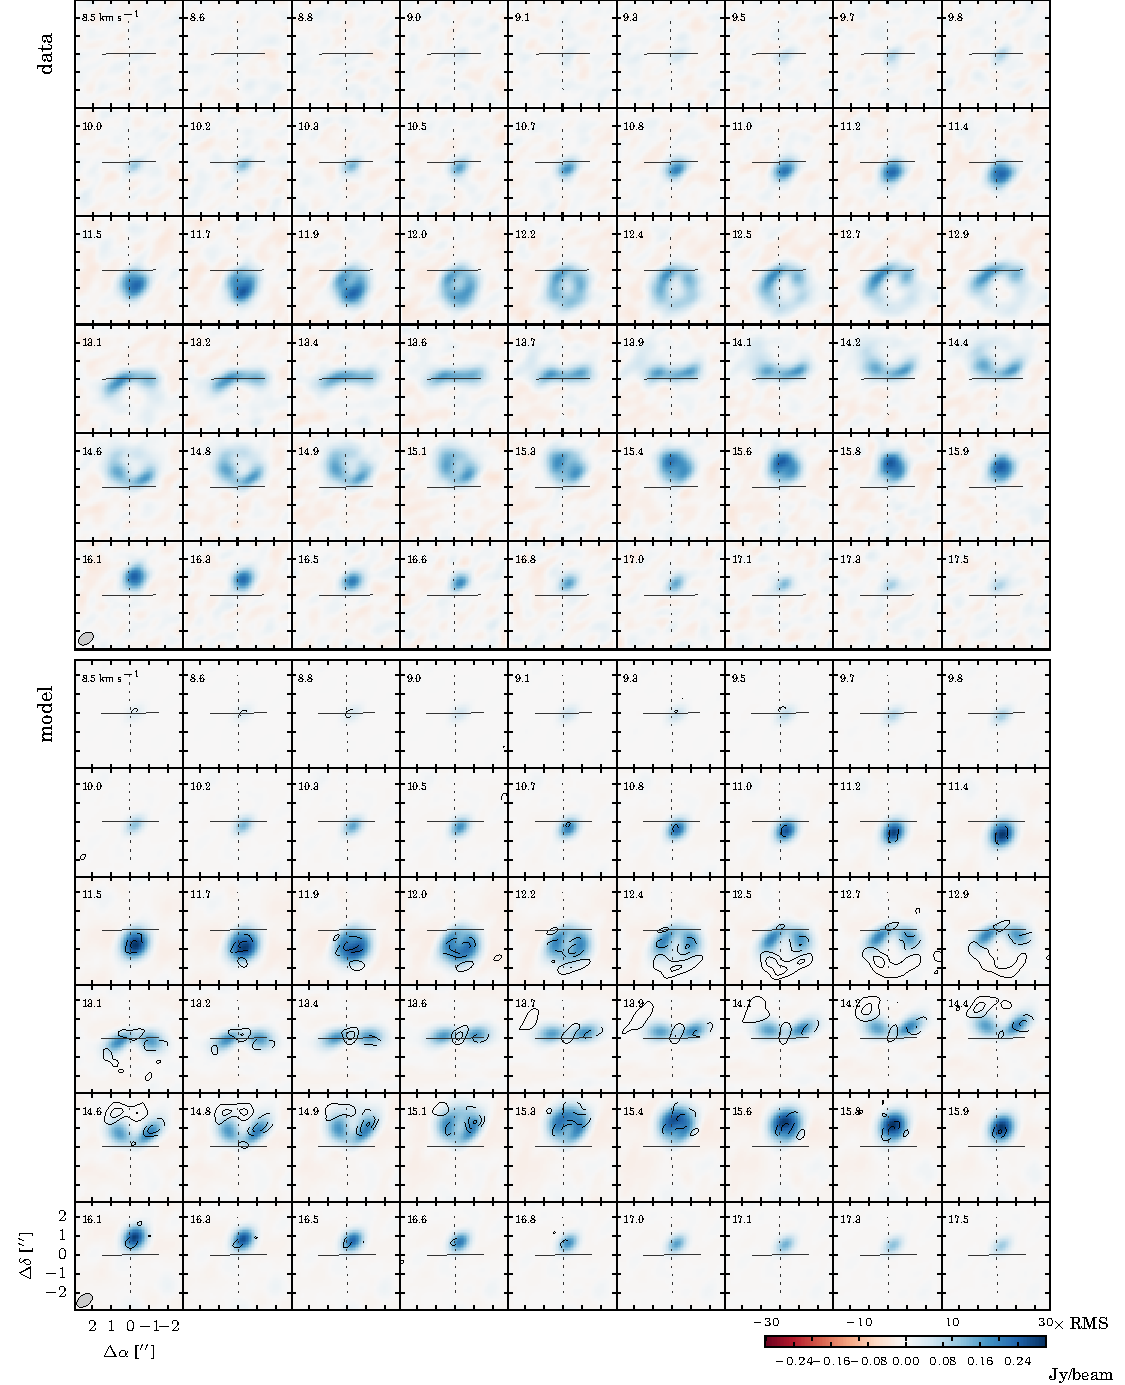
\includegraphics{chmaps_13CO.pdf}
  \figcaption{\thirteen\ channel maps, model, and residuals.
  \label{fig:chmaps_13CO}}
  \end{center}
\end{figure*}

\begin{figure*}[htb]
\begin{center}
  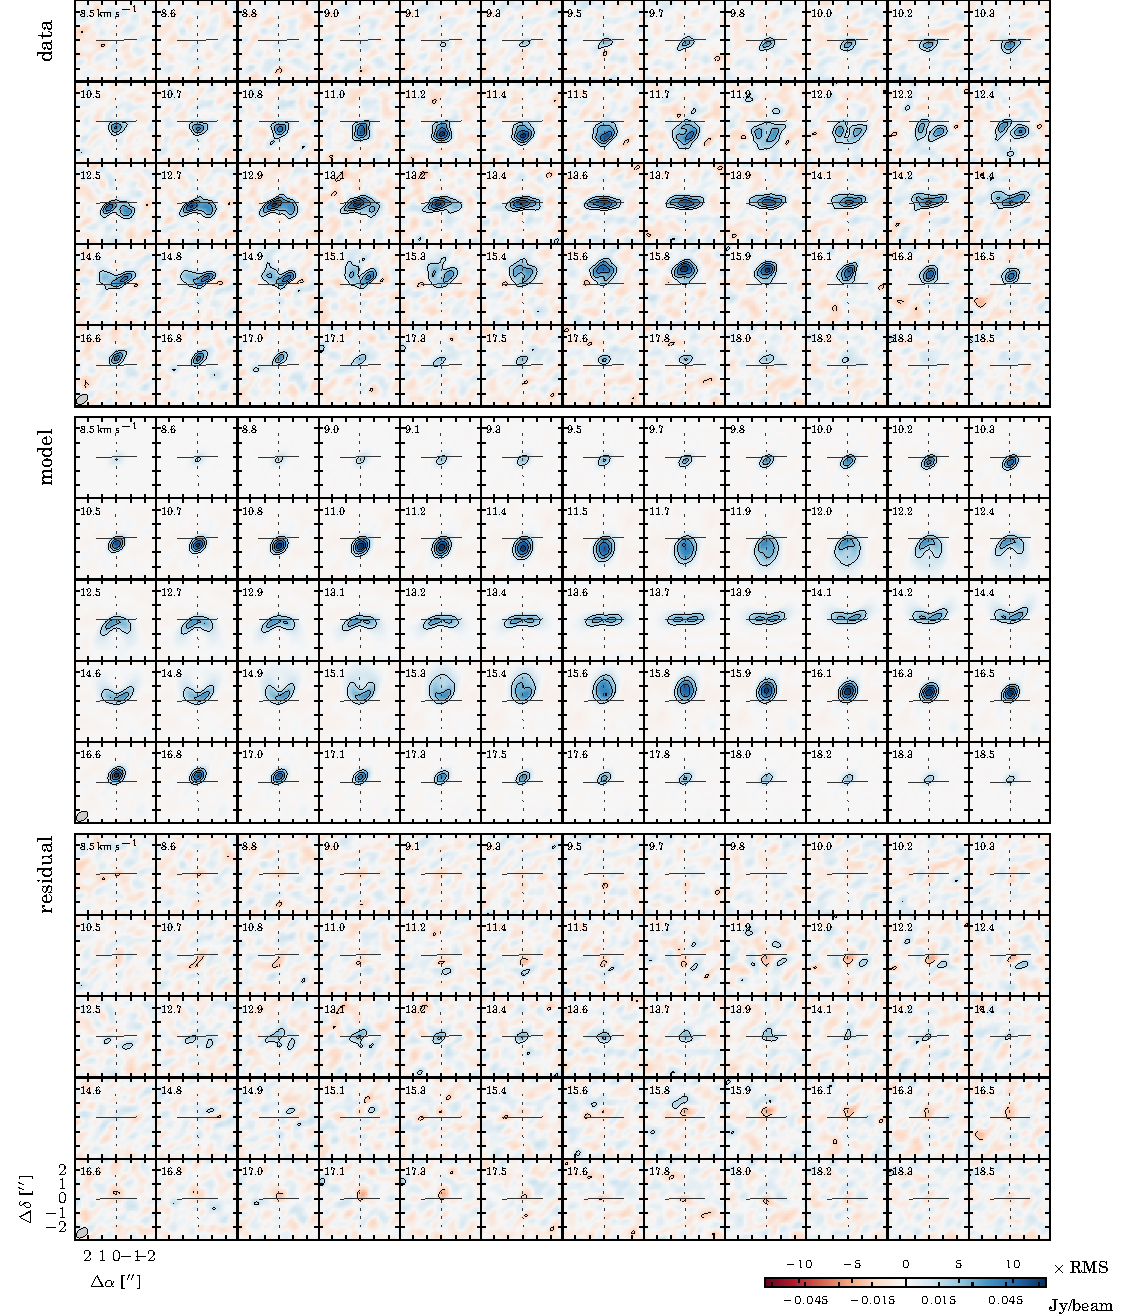
\includegraphics{chmaps_C18O.pdf}
  \figcaption{\eighteen\ channel maps, model, and residuals.
  \label{fig:chmaps_C18O}}
  \end{center}
\end{figure*}


\subsection{Spectroscopic Observations}

TRES and Digital Spedometer Observations.

\subsection{Photometric Observations}

Photometry from Grankin, KELT.

\section{Analysis and Results}

\subsection{CO Disk Modeling}

% Discussion of why we are using a model with vertical temperature gradient, does better job of explaining disk residuals.

% Inferred central mass
% Discussion of fit residuals
% Agreement across transitions

We analyze the \twelve, \thirteen, and \eighteen\ molecular line emission with the \texttt{DiskJockey} package \citep{czekala15a}\footnote{Open source under an MIT license at \url{https://github.com/iancze/DiskJockey}.}. Briefly, the package works to forward-model millimeter interferometric observations of molecular line emission with a parametric description of the disk structure, temperature, and velocity field. For a given set of parameters, the excellent radiative transfer package \texttt{RADMC-3D} \citep{dullemond12} is used to solve the radiative transfer equation and generate high-resolution channel maps. These images are then Fourier transformed and sampled at the same $u-v$ locations as the ALMA observations. The goodness of fit for each model is evaluated using a $\chi^2$ likelihood function which incorporates the visibility weights determined from the radiometer equation. After multiplying by the priors (discussed below), this posterior distribution is explored using the ensemble sampler MCMC \citep{goodman10,foreman-mackey13}.

Further model details about the standard setup of our modeling approach can be found in \citep{czekala15a,czekala16}. Motivated by the excellent quality of the well-resolved observations of multiple CO isotopologues, we extend the package to include a disk model with a vertical temperature gradient \citep[e.g.,][]{dartois03}. Instead of previously assuming that the temperature at each radius is vertically isothermal, we now include a parameterization \citep[following][]{rosenfeld13a,williams14} that allows a smooth transition from a ``midplane'' temperature to an ``atmosphere'' temperature. These two boundary temperatures are described by power laws
\begin{equation}
	T_m(r) = T_{m,10} \left ( \frac{r}{10\,\textrm{AU}} \right )^{-q_m}
\end{equation}

\begin{equation}
	T_a(r) = T_{a,10} \left ( \frac{r}{10\,\textrm{AU}} \right )^{-q_a}.
\end{equation}
The height of the atmosphere, $z_q$ is calculated as a multiple $h$ of the disk scale height $z_q(r) = h H(r)$, where for this analysis we fix $h = 4$. Between the midplane ($z = 0$) and atmosphere, the temperature is given by
\begin{equation}
	T(r, z) = T_m + (T_a - T_m)  \sin \left [ \frac{\pi z}{2 z_q} \right ]^{2 \delta}
\end{equation}
where we fix $\delta = 2$. At altitudes above $z_q$, the disk is again isothermal $T(r, z > z_q) = T_a(r)$. Because we are now considering large heights above the midplane, we properly calculate the velocity as the radial distance to the central stellar mass
\begin{equation}
	v^2(r, z) = \frac{G M_\ast}{(r^2 + z^2)^{1/2}}
\end{equation}
The radial surface density profile of the disk is still set by the density prescription of $\Sigma(r)$, however now the vertical density structure must be found by solving the equation for (vertical) hydrostatic equilibrium
\begin{equation}
	\frac{\partial \ln \rho}{\ln z} = - \left [\left (\frac{G M_\ast z}{(r^2 + z^2)^{3/2}} \right) \left ( \frac{\mu m_H}{k T} \right ) + \frac{\partial \ln T}{\partial z} \right].
\end{equation}
This ordinary differential equation (ODE) is solved numerically to yield an unnormalized vertical density profile. The normalization is given by the condition that $\Sigma(r) = \int_{-\infty}^{+\infty} \rho(r, z)\, \mathrm{d}z$, which is found by numerically integrating the solution to the ODE. We include a photodissociation threshold, wherever the column density of gas above a height is below \todo{XX}, we set the CO abundance to zero. This height $z_\mathrm{phot}$ is found by the solution to the equation $\sigma_\mathrm{phot}(r) = \int_{z_\mathrm{phot}}^\infty \rho(r, z)\, \mathrm{d}z.$

Lastly, we account for CO freezeout on to dust grains by decreasing the CO abundance by a factor of $100$ wherever the disk temperature is below $19\,$K. Because the distance to GW~Ori has been precisely determined by \citet{menten07} to be $414 \pm 7\,\textrm{pc}$, we order reduce the dimensionality of the problem and save computational time by exploring the model parameters with the distance to the source fixed at $d=414\,$pc. Because uncertainty in the source distance folds into uncertainty on $M_\ast$ in a linear manner, this is a small effect on the precision of $M_\ast$ compared to the statistical errors from the CO analysis.

\subsection{Updated Spectroscopic Orbit}

\begin{figure}[htb]
\begin{center}
  \includegraphics[draft,width=\textwidth,height=0.4\textheight]{orbit.pdf}
  \figcaption{Updated spectroscopic orbit.
  \label{fig:RV}}
  \end{center}
\end{figure}

RV variation of ~8-10 km/s coincides with an eclipse of ~0.6 mags in R, roughly gray. Might be caused by a knife-edge that has asymmetry wrt rotation axis (R-M effect).

Combining the RV constraints and disk constraints, we have the following constraints on component masses
\begin{deluxetable}{lr@{\,$\pm$\,}ll}
% \tabletypesize{font size command}
% \rotate
% \tablewidth{dimen}
% \tablenum{text}
% \tablecolumns{6}
\tablecaption{Combined disk and RV constraints on component masses\label{table:components}}
\tablehead{\colhead{Parameter} & \multicolumn{2}{c}{Value} & \colhead{Unit}}
\startdata
$M_\mathrm{tot}$ & 5.50 & 0.20 & $M_\odot$ \\
$i_\mathrm{d}$ & 135 & 2 & degrees \\
$M_A$ & 4.40 & 0.18 & $M_\odot$ \\
$M_B$ & 0.42 & 0.02 & $M_\odot$ \\
$M_C$ & 0.68 & 0.05 & $M_\odot$ \\
\enddata
\end{deluxetable}


\subsection{Expanded Catalog of Photometric Eclipses}

% Presentation of photometry.
% Catalog of eclipse dates
% Discussion of possible occultor radius

\begin{figure}[htb]
\begin{center}
  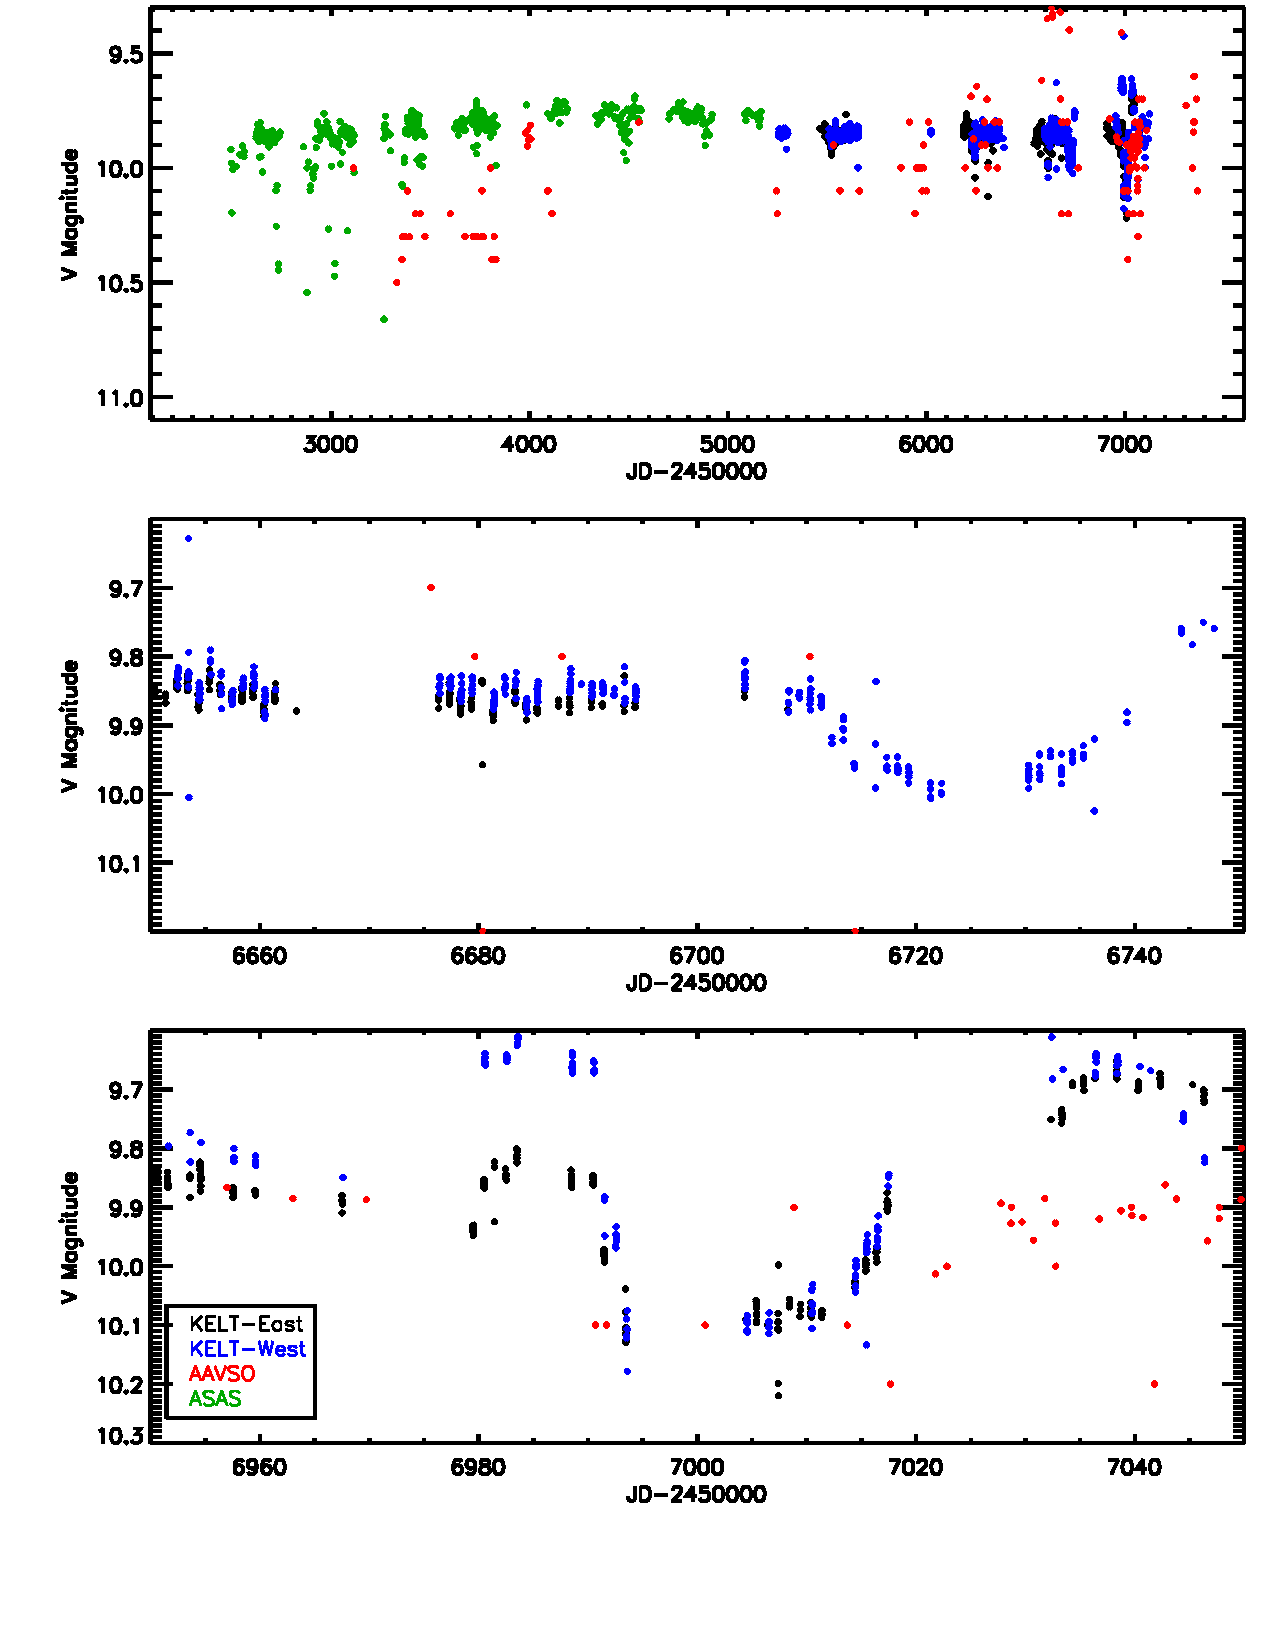
\includegraphics[height=0.5\textheight]{KELT_eclipses.pdf}
  \figcaption{
 KELT eclipses.
  \label{fig:KELT}}
  \end{center}
\end{figure}

Eclipses \citep{shevchenko92,shevchenko98}.

\begin{deluxetable}{rrrrrl}
% \tabletypesize{font size command}
% \rotate
% \tablewidth{dimen}
% \tablenum{text}
% \tablecolumns{6}
\tablecaption{Photometric Eclipse Catalog\label{table:eclipses} \todo{NOTE: this eclipse data is only for reference when doing the RV fit to exclude outliers. NOT for publication until appropriate authors (Shevchenko et al.) have been contacted and their permission granted.}
}
\tablehead{\colhead{Eclipse Number} & \colhead{Start} & \colhead{End} & \colhead{Duration} & \colhead{Decrement} & \colhead{Telescope}\\
& [JD] & [JD] & [days] & [mmag] &
}
\startdata
\nodata & 2447043 & 2447056 & 13 & 600 & \nodata \\
\nodata & 2447153 & 2447179 & 26 & 300 & \nodata \\
\nodata & 2447418 & 2447435 & 17 & 450 & \nodata \\
\nodata & 2447809 & 2447824 & 15 & 130 & \nodata \\
\nodata & 2448137 & 2448162 & 25 & 300 & \nodata \\
\nodata & 2448545 & 2448586 & 41 & 150 & \nodata \\
\nodata & $\geq$2450399 & $\leq$2450414 & $\leq$15 & 300 & \nodata \\
\nodata & 2452184 & $\geq$2452209 & $\geq$ 25 & 750 & \nodata \\
\nodata & 2456710 & 2456744 & 34 & 130 & KELT \\
\nodata & 2456989 & 2457030 & $\leq$41 & 220 & KELT \\ % Nov 28th, 2014
\enddata
\end{deluxetable}

Figure from KELT, ASAS, and AAVSO.

\section{Discussion}

\subsection{Evolutionary status of GW Ori components}
Discussion of our inferred component masses with that of \citet{berger11}.

Photospheric analysis of properties (based on either spectral type + SED of primary and/or limits on the secondary) coupled with 4 usual PMS models and \citet{choi16} models.

\begin{figure}[htb]
\begin{center}
  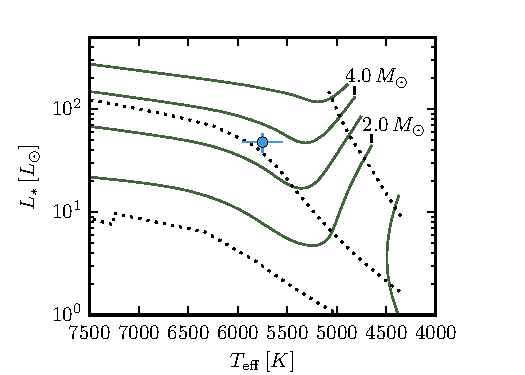
\includegraphics{tracks.pdf}
  \figcaption{MIST PMS tracks
  \label{fig:PMS}}
  \end{center}
\end{figure}

Figure showing evolution of photospheric properties as a function of time.

Discussion of component masses relative to ideas about formation, migration.

\subsection{GW Ori as a triple system}

{\it Some notes from Eric from reading literature on what is known about triple systems.  Is this extreme?}

While the ratio between the outer orbital period and the inner orbital period is smaller than in many hierarchical systems, it is not an outlier among triple systems.  In a detailed analysis of higher-order multiple systems, \citet{tokovinin97} found that the ratio $P_{\rm long} / P_{\rm short}$ in almost all systems was greater than 10, presumably reflecting which orbits are stable.  In GW Ori, this ratio is 16.

(Tokovinin has an updated catalog on his website with about twice as many systems as in the CDS version from this paper, but it would be non-trivial to figure out how to remake the above plot.  Not sure it's necessary.)

Among late B star primaries (which GW Ori Aa will be on the main sequence), 13\% of systems have multiplicity of three or higher \citep{eggleton08}; this fraction is roughly constant across spectral types B--G.

\citet{tokovinin97} finds that the distribution of mutual inclinations of the orbits in triple systems is inconsistent both with complete alignment of the inner and outer orbits, but also with independent inclinations of the two orbits.  However, we should note that this is for a population of much older systems, in which significant dynamical evolution could have occurred, particularly for the shorter-period systems.  The fact that GW Ori appears to have roughly-aligned, circular inner and outer orbits (!! does it?  to be confirmed) is suggestive of formation of one or both companions from the massive disk surrounding the system.  (Wild speculation here.)

Offner et al 2010 is probably important for us to look at regarding fragmentation vs.\ disk instability.  They also cite Howe \& Clarke 2009 for a review of observations.

Bate 2012 on his big fragmentation simulation: ``In particular, despite the fact that no objects form closer than $\approx 10$ au from each other, at the end of the calculation there exist 21 binary systems and one triple system with separations $<10$ au.''

In his simulations, of the triples that form, the orbits are misaligned with each other (though three are $\leq 6$ degrees, and 8 out of 9 are $\leq 36$ degrees).

Bate:  ``Observations also indicate that eccentricities $e < 0.1$ are rare for periods greater than $\approx$ 100 d (separations $\gtrsim$ 1 au). Raghavan et al. (2010) find no binaries with $e < 0.1$ and orbital periods greater than 100 d, though they do find that the outer orbits of two triples and one quadruple have $e < 0.1$. Duquennoy \& Mayor (1991) and Raghavan et al. (2010) also find that the upper-eccentricity envelope is dominated by components of triple systems, possibly due to the action of the Kozai mechanism (Kozai 1962).''

Important for us to see what constraints we have on eccentricity of the orbits.

Speculation from \citet{berger11} about whether this system is actual stable.

\section{Summary and Conclusions} \label{sec:summary}

\acknowledgments
IC is supported by the Smithsonian Institution. IC acknowledges helpful conversations with Maxwell Moe about GW Ori and related systems.  SA acknowledges the very helpful support provided by the NRAO Student Observing Support program related to the early development of this project.  This paper makes use of the following ALMA data: XX  ALMA is a partnership of ESO (representing its member states), NSF (USA), and NINS (Japan), together with NRC (Canada) and NSC and ASIAA (Taiwan), in cooperation with the Republic of Chile.  The Joint ALMA Observatory is operated by ESO, AUI/NRAO, and NAOJ.  This research made extensive use of the Julia programming language \citep{julia12} and Astropy \citep{astropy13}.

\bibliographystyle{aasjournal.bst}
\bibliography{GWOri.bib}

\end{document}
